\section{Jeux d'essais}

    Cette partie présente les principales fonctionnalités de l'application au travers de captures d'écrans.
    
    \paragraph{}
    L'image~\ref{fig:lancement_serveur} ci-dessous montre l'écran affiché lors du démarrage du serveur. On peut voir le numéro de port à utiliser : 5000.
    \begin{figure}[!htpb]
        \centering
        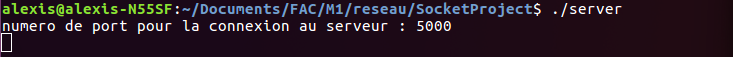
\includegraphics[width=10cm]{captures/lancement_serveur.png}
        \caption{\textit{Démarrage du serveur}}
        \label{fig:lancement_serveur}
    \end{figure}
    
    \FloatBarrier
    
    \paragraph{}
    L'image~\ref{fig:lancement_client} ci-dessous montre l'écran de démarrage d'un client se connectant au serveur. On peut apercevoir le message "test s'est connecté", ce qui montre bien que la connexion est réussie.
    \begin{figure}[!htpb]
        \centering
        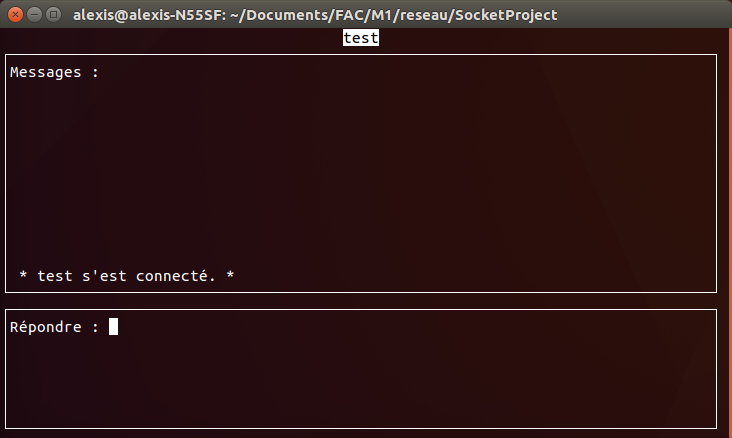
\includegraphics[width=10cm]{captures/lancement_client.png}
        \caption{\textit{Démarrage du client}}
        \label{fig:lancement_client}
    \end{figure}
    
    \FloatBarrier
    
    \paragraph{}
    L'image~\ref{fig:erreur_connexion} ci-dessous montre le message d'erreur affiché lorsque les paramètres de connexion chez le client sont mal renseignés.
    \begin{figure}[!htpb]
        \centering
        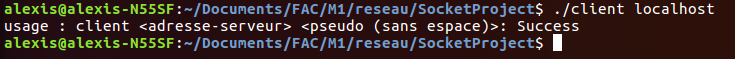
\includegraphics[width=10cm]{captures/erreur_connexion.png}
        \caption{\textit{Erreur de connexion}}
        \label{fig:erreur_connexion}
    \end{figure}
    
    \FloatBarrier
    
    \paragraph{}
    L'image~\ref{fig:connexion_serveur} ci-dessous montre que le client "test" s'est connecté sur le serveur et possède le numéro de socket "4".
    \begin{figure}[!htpb]
        \centering
        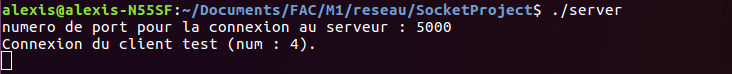
\includegraphics[width=10cm]{captures/connexion_serveur.png}
        \caption{\textit{Connexion sur le serveur}}
        \label{fig:connexion_serveur}
    \end{figure}
    
    \FloatBarrier
    
    \paragraph{}
    L'image~\ref{fig:cmd_help} ci-dessous montre le résultat de la commande "help".
    \begin{figure}[!htpb]
        \centering
        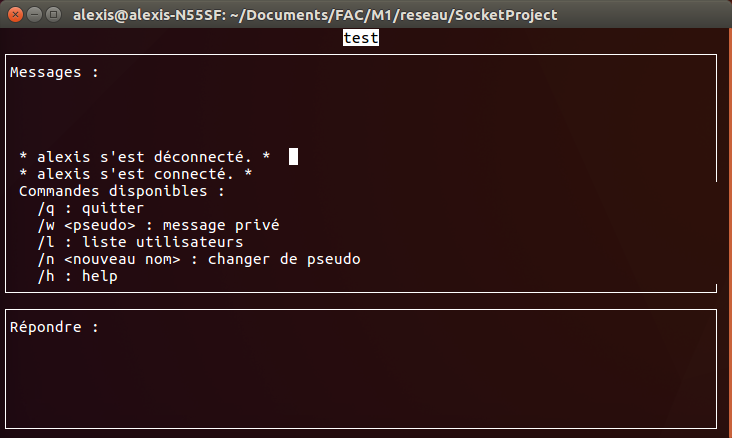
\includegraphics[width=10cm]{captures/cmd_help.png}
        \caption{\textit{Commande /h}}
        \label{fig:cmd_help}
    \end{figure}
    
    \FloatBarrier
    
    \paragraph{}
    L'image~\ref{fig:cmd_liste_utilisateurs} ci-dessous montre le résultat de la commande "liste utilisateurs". Ici trois utilisateurs sont connectés au serveur.
    \begin{figure}[!htpb]
        \centering
        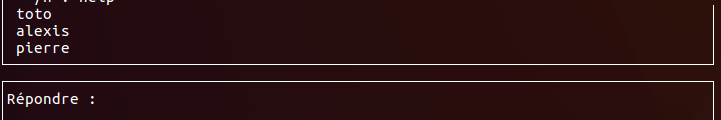
\includegraphics[width=10cm]{captures/cmd_liste_utilisateurs.png}
        \caption{\textit{Commande /l}}
        \label{fig:cmd_liste_utilisateurs}
    \end{figure}
    
    \FloatBarrier
    
    \paragraph{}
    L'image~\ref{fig:cmd_mp} ci-dessous montre le résultat de la commande "message privé" suivi du pseudo du destinataire : "alexis".
    \begin{figure}[!htpb]
        \centering
        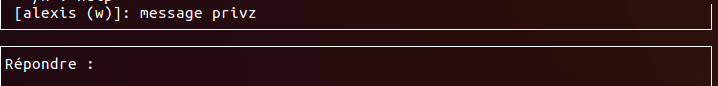
\includegraphics[width=10cm]{captures/cmd_mp.png}
        \caption{\textit{Commande /w}}
        \label{fig:cmd_mp}
    \end{figure}
    
    \FloatBarrier
    
    \paragraph{}
    L'image~\ref{fig:cmd_mp_erreur} ci-dessous montre le résultat de la commande "message privé" avec une erreur : "Le client n'existe pas".
    \begin{figure}[!htpb]
        \centering
        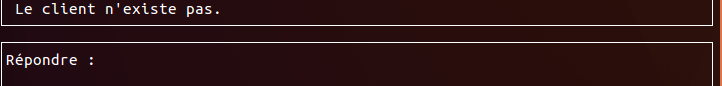
\includegraphics[width=10cm]{captures/cmd_mp_erreur.png}
        \caption{\textit{Commande /w avec erreur}}
        \label{fig:cmd_mp_erreur}
    \end{figure}
    
    \FloatBarrier
    
    \paragraph{}
    L'image~\ref{fig:cmd_renommage} ci-dessous montre le résultat de la commande "changer de pseudo" suivi du pseudo "toto".
    \begin{figure}[!htpb]
        \centering
        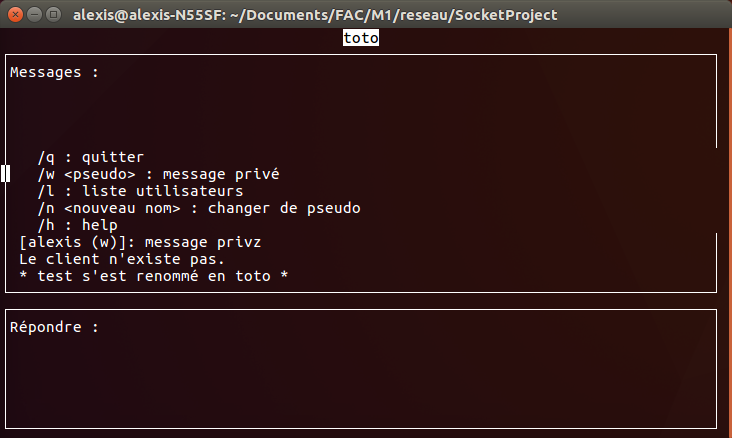
\includegraphics[width=10cm]{captures/cmd_renommage.png}
        \caption{\textit{Commande /n}}
        \label{fig:cmd_renommage}
    \end{figure}
    
    \FloatBarrier
    
    \paragraph{}
    L'image~\ref{fig:deconnexion_client} ci-dessous montre la déconnexion d'un autre client (ici la déconnexion de toto).
    \begin{figure}[!htpb]
        \centering
        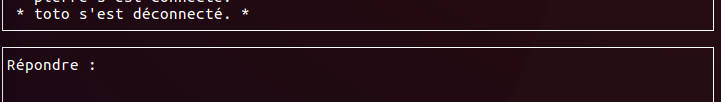
\includegraphics[width=10cm]{captures/deconnexion_client.png}
        \caption{\textit{Déconnexion d'un client}}
        \label{fig:deconnexion_client}
    \end{figure}
    
    \FloatBarrier
    
    \paragraph{}
    L'image~\ref{fig:deconnexion_serveur} ci-dessous montre la déconnexion de toto sur le serveur. Le numéro de socket "4" est désormais disponible.
    \begin{figure}[!htpb]
        \centering
        
\includegraphics[width=10cm]{captures/deconnexion_serveur.png}
        \caption{\textit{Déconnexion d'un client (vue serveur)}}
        \label{fig:deconnexion_serveur}
    \end{figure}